\subsection{Walking model}\label{walkingmodel}

In \cite{Seyfarth2006}, a model of two compliant legs is proposed. In this model, when one leg is on the ground, the system is equivalent to a inverted spring pendulum, this is called the single support phase. When the model is not in a single support phase, it is in a double support phase, where the two springs in this phase influence the movement of the CoM at the same time, reproducing a bipedal spring-mass walking. The springs accumulate and deliver energy so that the system remains convervative with no energy losses.

\noindent In single phase support, the dynamics of the center of mass (CoM) is as follows,
\begin{equation}
  \ddot{x}=\frac{F_1}{m}\frac{x-x_{t1}}{l_1},
  \label{eq.singlesuppx}
  \end{equation}
\begin{equation}
  \ddot{y}=\frac{F_1}{m}\frac{y-y_{t1}}{l_1}-g,
  \label{eq.singlesuppy}
\end{equation}
 where $(x,y)$ are the coordinates of the center of mass (CoM  and $(x_{ti},y_{ti})$ are the coordenates of the respective toes for the leg 1 and leg 2.
\noindent With double support, the dynamics are similar to the previous case with the difference that we are in the presence of two springs, this is,
\begin{equation}
 \ddot{x}=\frac{F_1}{m}\frac{x-x_{t1}}{l_1}+\frac{F_2}{m}\frac{x-x_{t2}}{l_2},
 \label{eq.doublesuppx}
  \end{equation}
\begin{equation}
  \ddot{y}=\frac{F_1}{m}\frac{y-y_{t1}}{l_1}+\frac{F_2}{m}\frac{y-y_{t2}}{l_2}-g,
  \label{eq.doublesuppy}
\end{equation}
with $F_i$ being the force applied on the mass by the respective leg,
\begin{equation}
  F_i=k(l_0-l_i)\geq 0 \,\,\,\,\, i=1,2\,,
\end{equation}
$l_0$ is the natural length of the spring, $l_i$ is the respective length,
\begin{equation}
l_i=\sqrt{(x-x_{ti})^2+(y-y_{ti})^2} \,\,\,\,\, i =1,2 \,.
\end{equation}
\noindent  Fig. (\ref{Seyfarthmodel}) illustrates the model, single support to double support transitions occur when the center of mass drops to a height of $y \sin{\alpha}$ where $\alpha$ is the angle of attack and the vertical velocity is negative. Double support to single support transitions occur when the spring deflection $l_0 - l_i$ of one of the legs return to 0.

Let the Poincaré section be defined as the vector $\psi_n=(y_n,\beta_n)^T$ at the Vertical Leg Orientation (VLO). Everytime the system is in the single support phase and the leg is in it's vertical position we record the height of the CoM, $y_n$ and the angle that the velocity makes with the ground, $\beta_n$. This state of the system defines the \textbf{stride} $n$ of the simulation. Alternatively a \textbf{step} is defined when the system passes from single support to double support.

\begin{figure}[H]
\centering
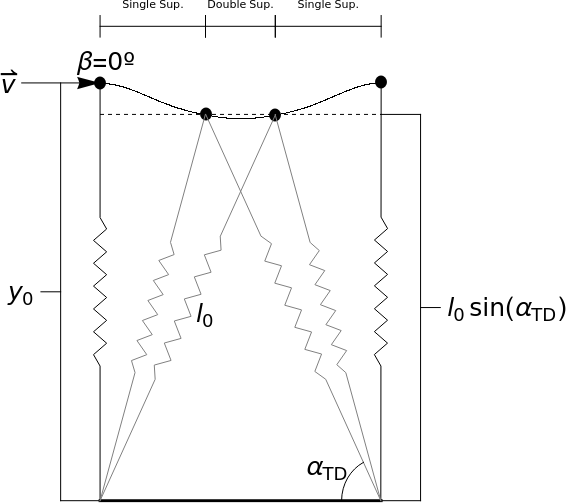
\includegraphics[width=0.7\textwidth]{Seyfarth2006_trimmed.png}
\caption{Bipedal spring-mass walking model described in \cite{Seyfarth2006}. The initial velocity is given by $\vec{v}$, in this case, $\beta=0$, this is the velocity is initially parallel to the ground, $\alpha_{TD}$ is the angle of attack for each leg, this is, the aperture that the leg has when it starts the double support phase. In this example, a step occurs when the system passes from single support to double support and a stride is defined when the leg  becomes aligned with the toe, this is , the leg returns to it's vertical leg orientation}
\label{Seyfarthmodel}
\end{figure}


This model is energetically conservative, therefore, the energy $E$ is a constant with

\begin{equation}
  E=\frac{k (l_0-y_n)^2}{2} + m g y_n + m \frac{v_n^2}{2}.
\end{equation}
\noindent We can express the absolute value of the velocity in terms of the energy. In this model, the only parameters in the initial conditions that can alter the stability of the system for a certain angle of attack $\alpha$, and energy $E$ are $\beta_0$, the angle of the initial velocity with the ground and $y_0$, the initial vertical position of the CoM.

By allowing the simulation to run over one stride/step, we can associate a map, which is called the Poincaré map, by defining a function $A$ which iterates the Poincaré section, $\psi_n=(y_n,\beta_n)$, this way,

\begin{equation}
  \psi_{n+1}=A \psi_n.
\end{equation}
By recurrence we can apply the $A$ function $n+1$ times from the initial state $\psi_0$ to get to the final step $n+1$.
Not all solutions are admited, if in any instance, the CoM ends up falling this is, $y<0$, or starts walking backwards, $v_x<0$, or the leg leaves the ground, $y>l_0$, the set of initial parameters is rejected as a possible stable combination.







